

\documentclass{article}

\usepackage[utf8]{inputenc}

\usepackage{amsmath, bm}
\usepackage{graphicx}
\usepackage{amssymb}
\usepackage{float}
\usepackage{caption}
\usepackage{subcaption}
\usepackage{hyperref}
\usepackage{tikz}
\usepackage{layout}

\usepackage[margin=1in]{geometry}
\usepackage{listings}
\usepackage{xcolor}
\usepackage{color, colortbl}
\usepackage{textgreek}
\usepackage{mathrsfs}
\usepackage{booktabs}

\usepackage{titlesec}

\titleformat{\subsubsection}
  {\normalfont\selectfont}{\thesubsubsection}{1em}{}

\usetikzlibrary{calc}
\usetikzlibrary{angles,quotes} % for pic
\usetikzlibrary{patterns,snakes}
\usetikzlibrary{arrows}
\tikzset{>=latex} % for LaTeX arrow head

\setlength{\parskip}{\baselineskip}%
\setlength{\parindent}{0pt}%
\linespread{0.9}


\definecolor{codegreen}{rgb}{0,0.6,0}
\definecolor{codegray}{rgb}{0.5,0.5,0.5}
\definecolor{codepurple}{rgb}{0.58,0,0.82}
\definecolor{backcolour}{rgb}{0.95,0.95,0.92}

\lstdefinestyle{mystyle}{
    backgroundcolor=\color{backcolour},   
    commentstyle=\color{codegreen},
    keywordstyle=\color{magenta},
    numberstyle=\tiny\color{codegray},
    stringstyle=\color{codepurple},
    basicstyle=\ttfamily\footnotesize,
    breakatwhitespace=false,         
    breaklines=true,                 
    captionpos=b,                    
    keepspaces=true,                 
    numbers=left,                    
    numbersep=5pt,                  
    showspaces=false,                
    showstringspaces=false,
    showtabs=false,                  
    tabsize=2
}

\lstset{style=mystyle}



\begin{document}

\title{4A4 Exercise 2}
\author{5739G}
\date{Feburary 2025}
\maketitle

\section{Introduction}

\iffalse
The equations of motion for surge, heave and pitch, in matrix form seen below.

\begin{equation}
  \frac{d}{dt}\left[\begin{matrix}u\\w\\\theta\\q\end{matrix}\right] = \left[\begin{matrix}\frac{X_{u}}{m} & \frac{X_{w}}{m} & - g & \frac{X_{q}}{m}\\\frac{Z_{u}}{m} & \frac{Z_{w}}{m} & 0 & \frac{U m + Z_{q}}{m}\\0 & 0 & 0 & 1\\\frac{M_{u}}{I_{y}} & \frac{M_{w}}{I_{y}} & 0 & 0\end{matrix}\right]
  \left[\begin{matrix}u\\w\\\theta\\q\end{matrix}\right] + 
  \left[\begin{matrix}0\\0\\0\\\frac{M_{\delta e}}{I_{y}}\end{matrix}\right]
  \left[\begin{matrix}\delta_{e}\end{matrix}\right]
\end{equation}

Which is in the state space form $\dot{\mathbf{x}} = \mathbf{Ax+Bu}
\fi

Real flight data was collected from inertial, pitot-static and avionic sensors onboard the SAAB 340B aircraft.
Intentional pilot control inputs were made to excite the aircrafts natural modes.

\section{Summary of Modes}

\begin{table}[H]
  \centering
  \begin{tabular}{lcc}
      \toprule
      Name & Damping factor & Natural frequency (rad/s) \\
      \midrule
      Phugoid & 0.06 & 0.126 \\
      Dutch Roll & 0.12 & 1.52 \\
      SPO & 0.429 & 2.23 \\
      \bottomrule
  \end{tabular}
  \caption{Oscillatory Modes \cite{e2}}
    \label{tab:oscillatory_modes}
\end{table}

\begin{table}[H]
  \centering
  \begin{tabular}{lc}
      \toprule
      Name & Time constant (s) \\
      \midrule
      Spiral & 30.31 \\
      Roll Subsidence & 1.52 \\
      \bottomrule
  \end{tabular}
  \caption{Non-Oscillatory Modes \cite{e2}}
  \label{tab:non_oscillatory_modes}
\end{table}


\begin{figure}[H]
    \centering
    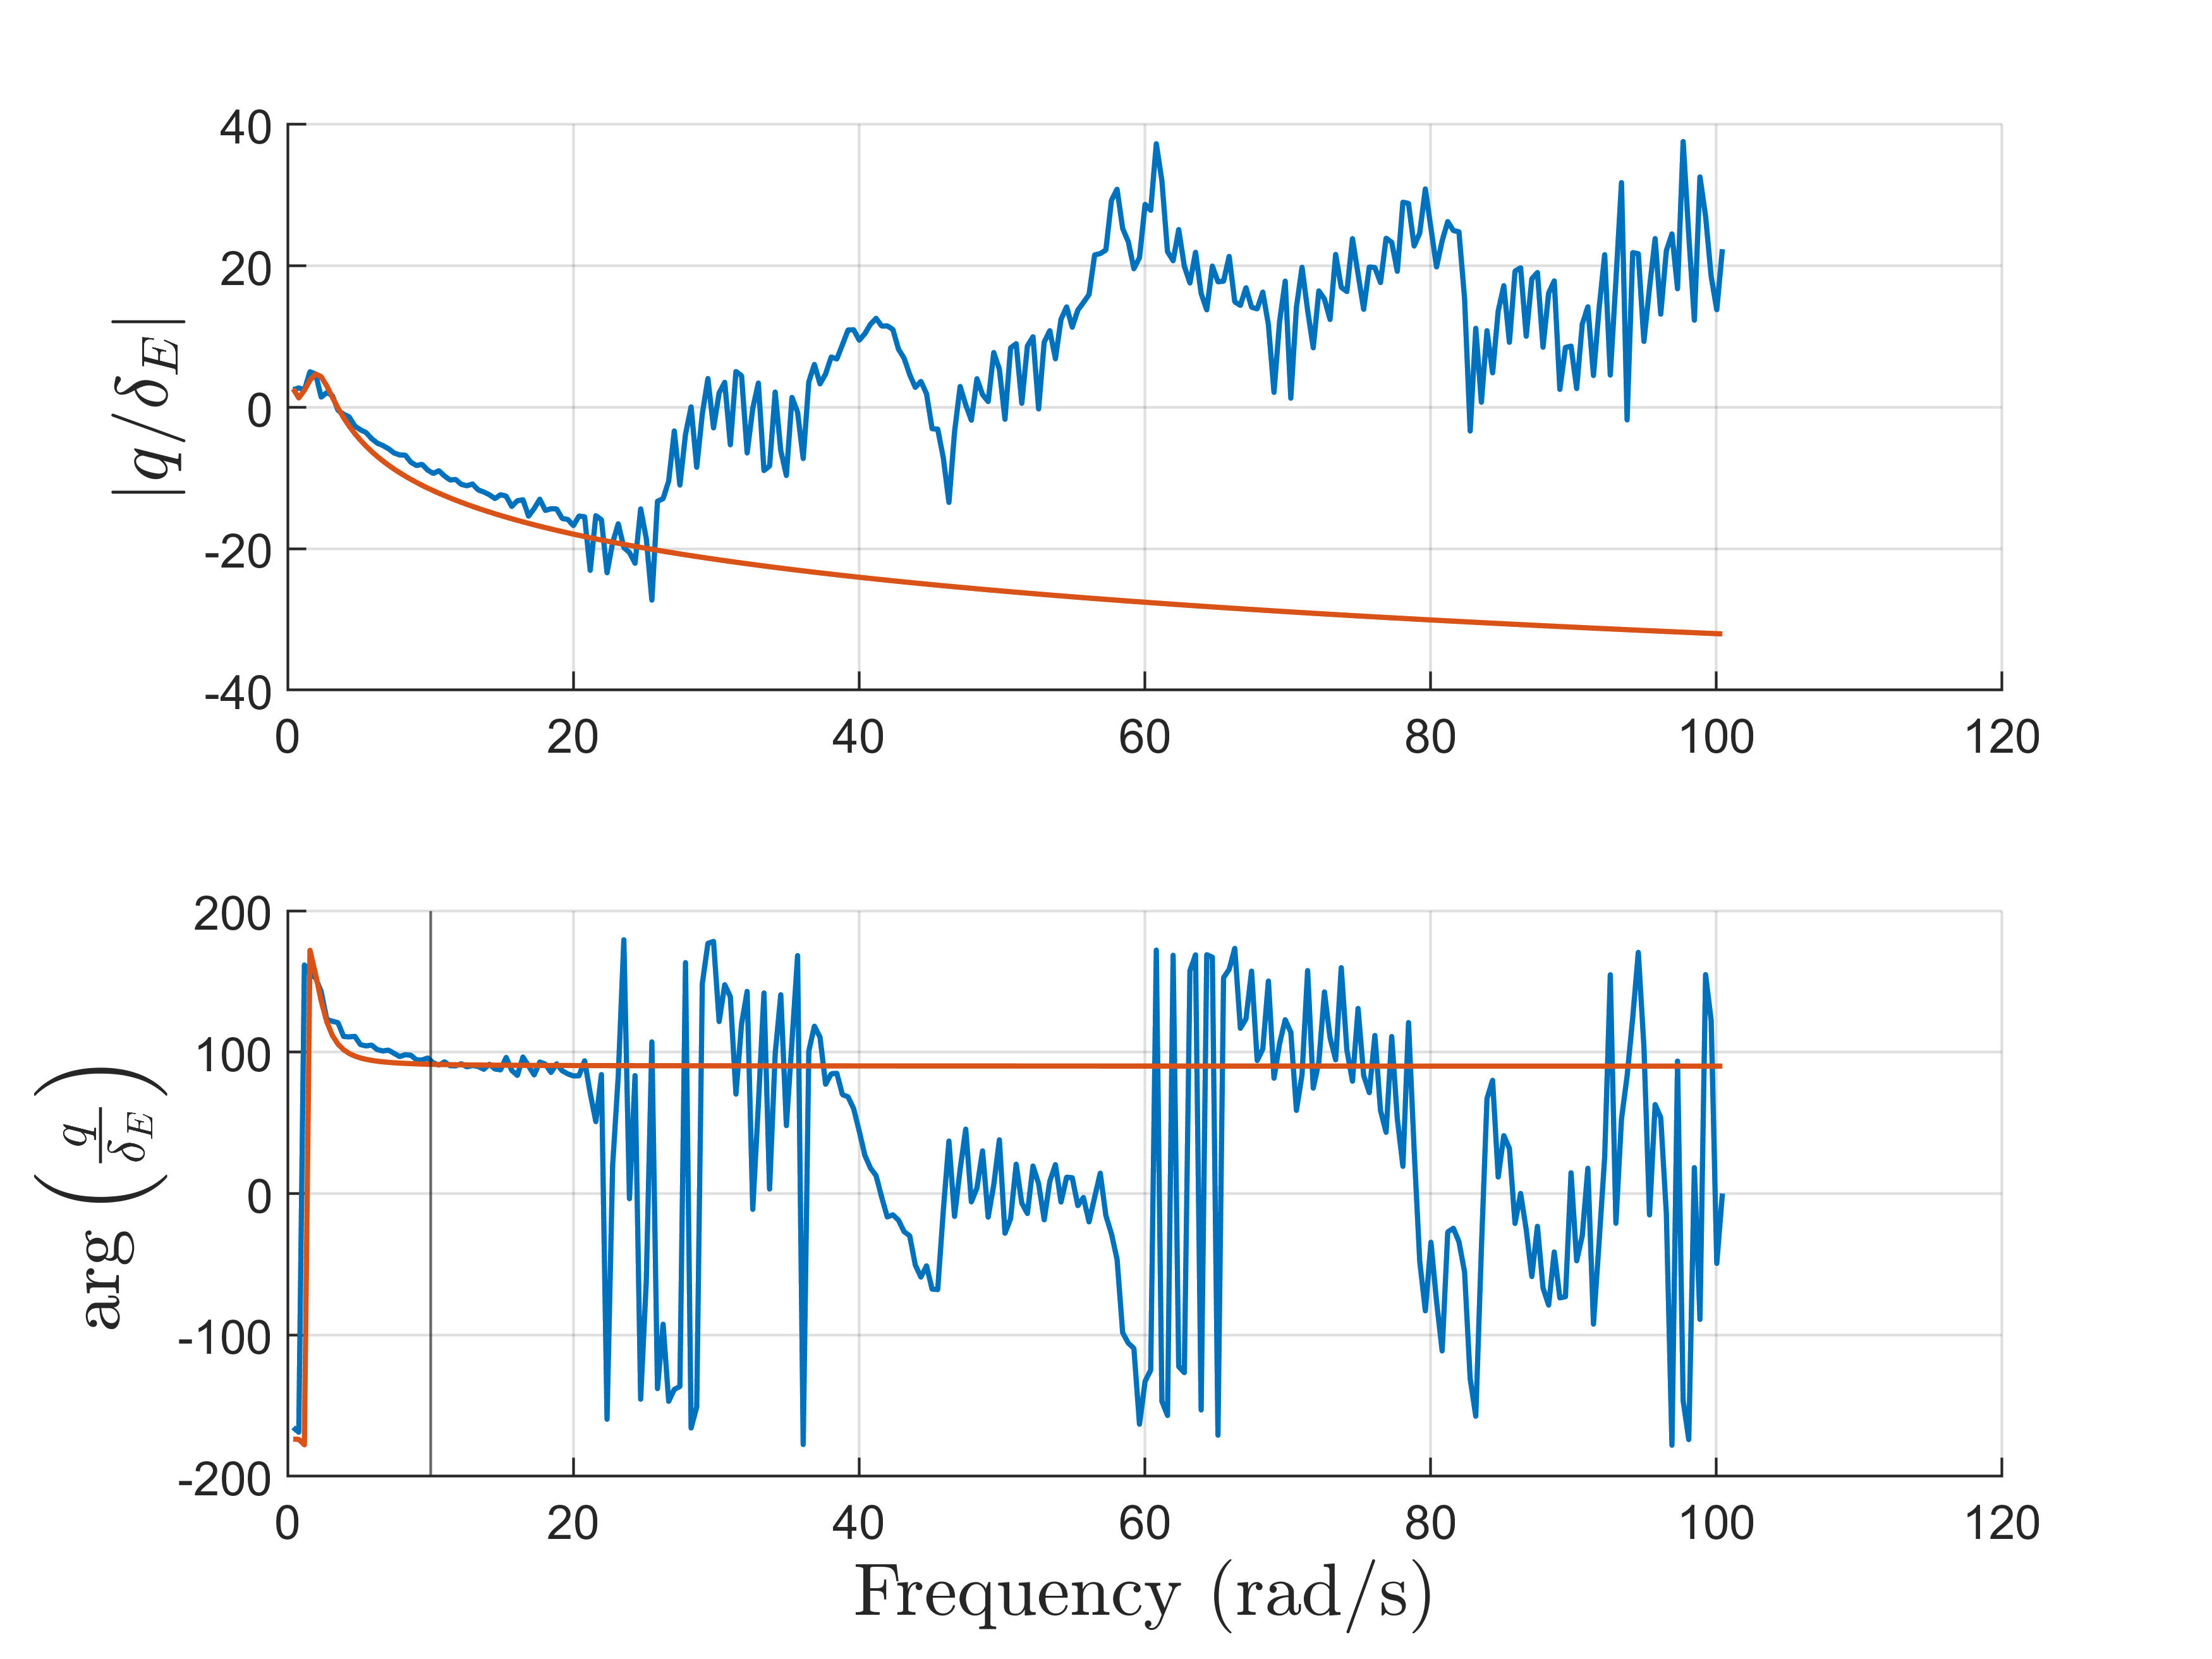
\includegraphics[width=0.6\textwidth]{elev_to_pitchrate.png}
    \caption{}
    \label{fig:elev_to_pitchrate}
  \end{figure}
  
  \begin{figure}[H]
      \centering
      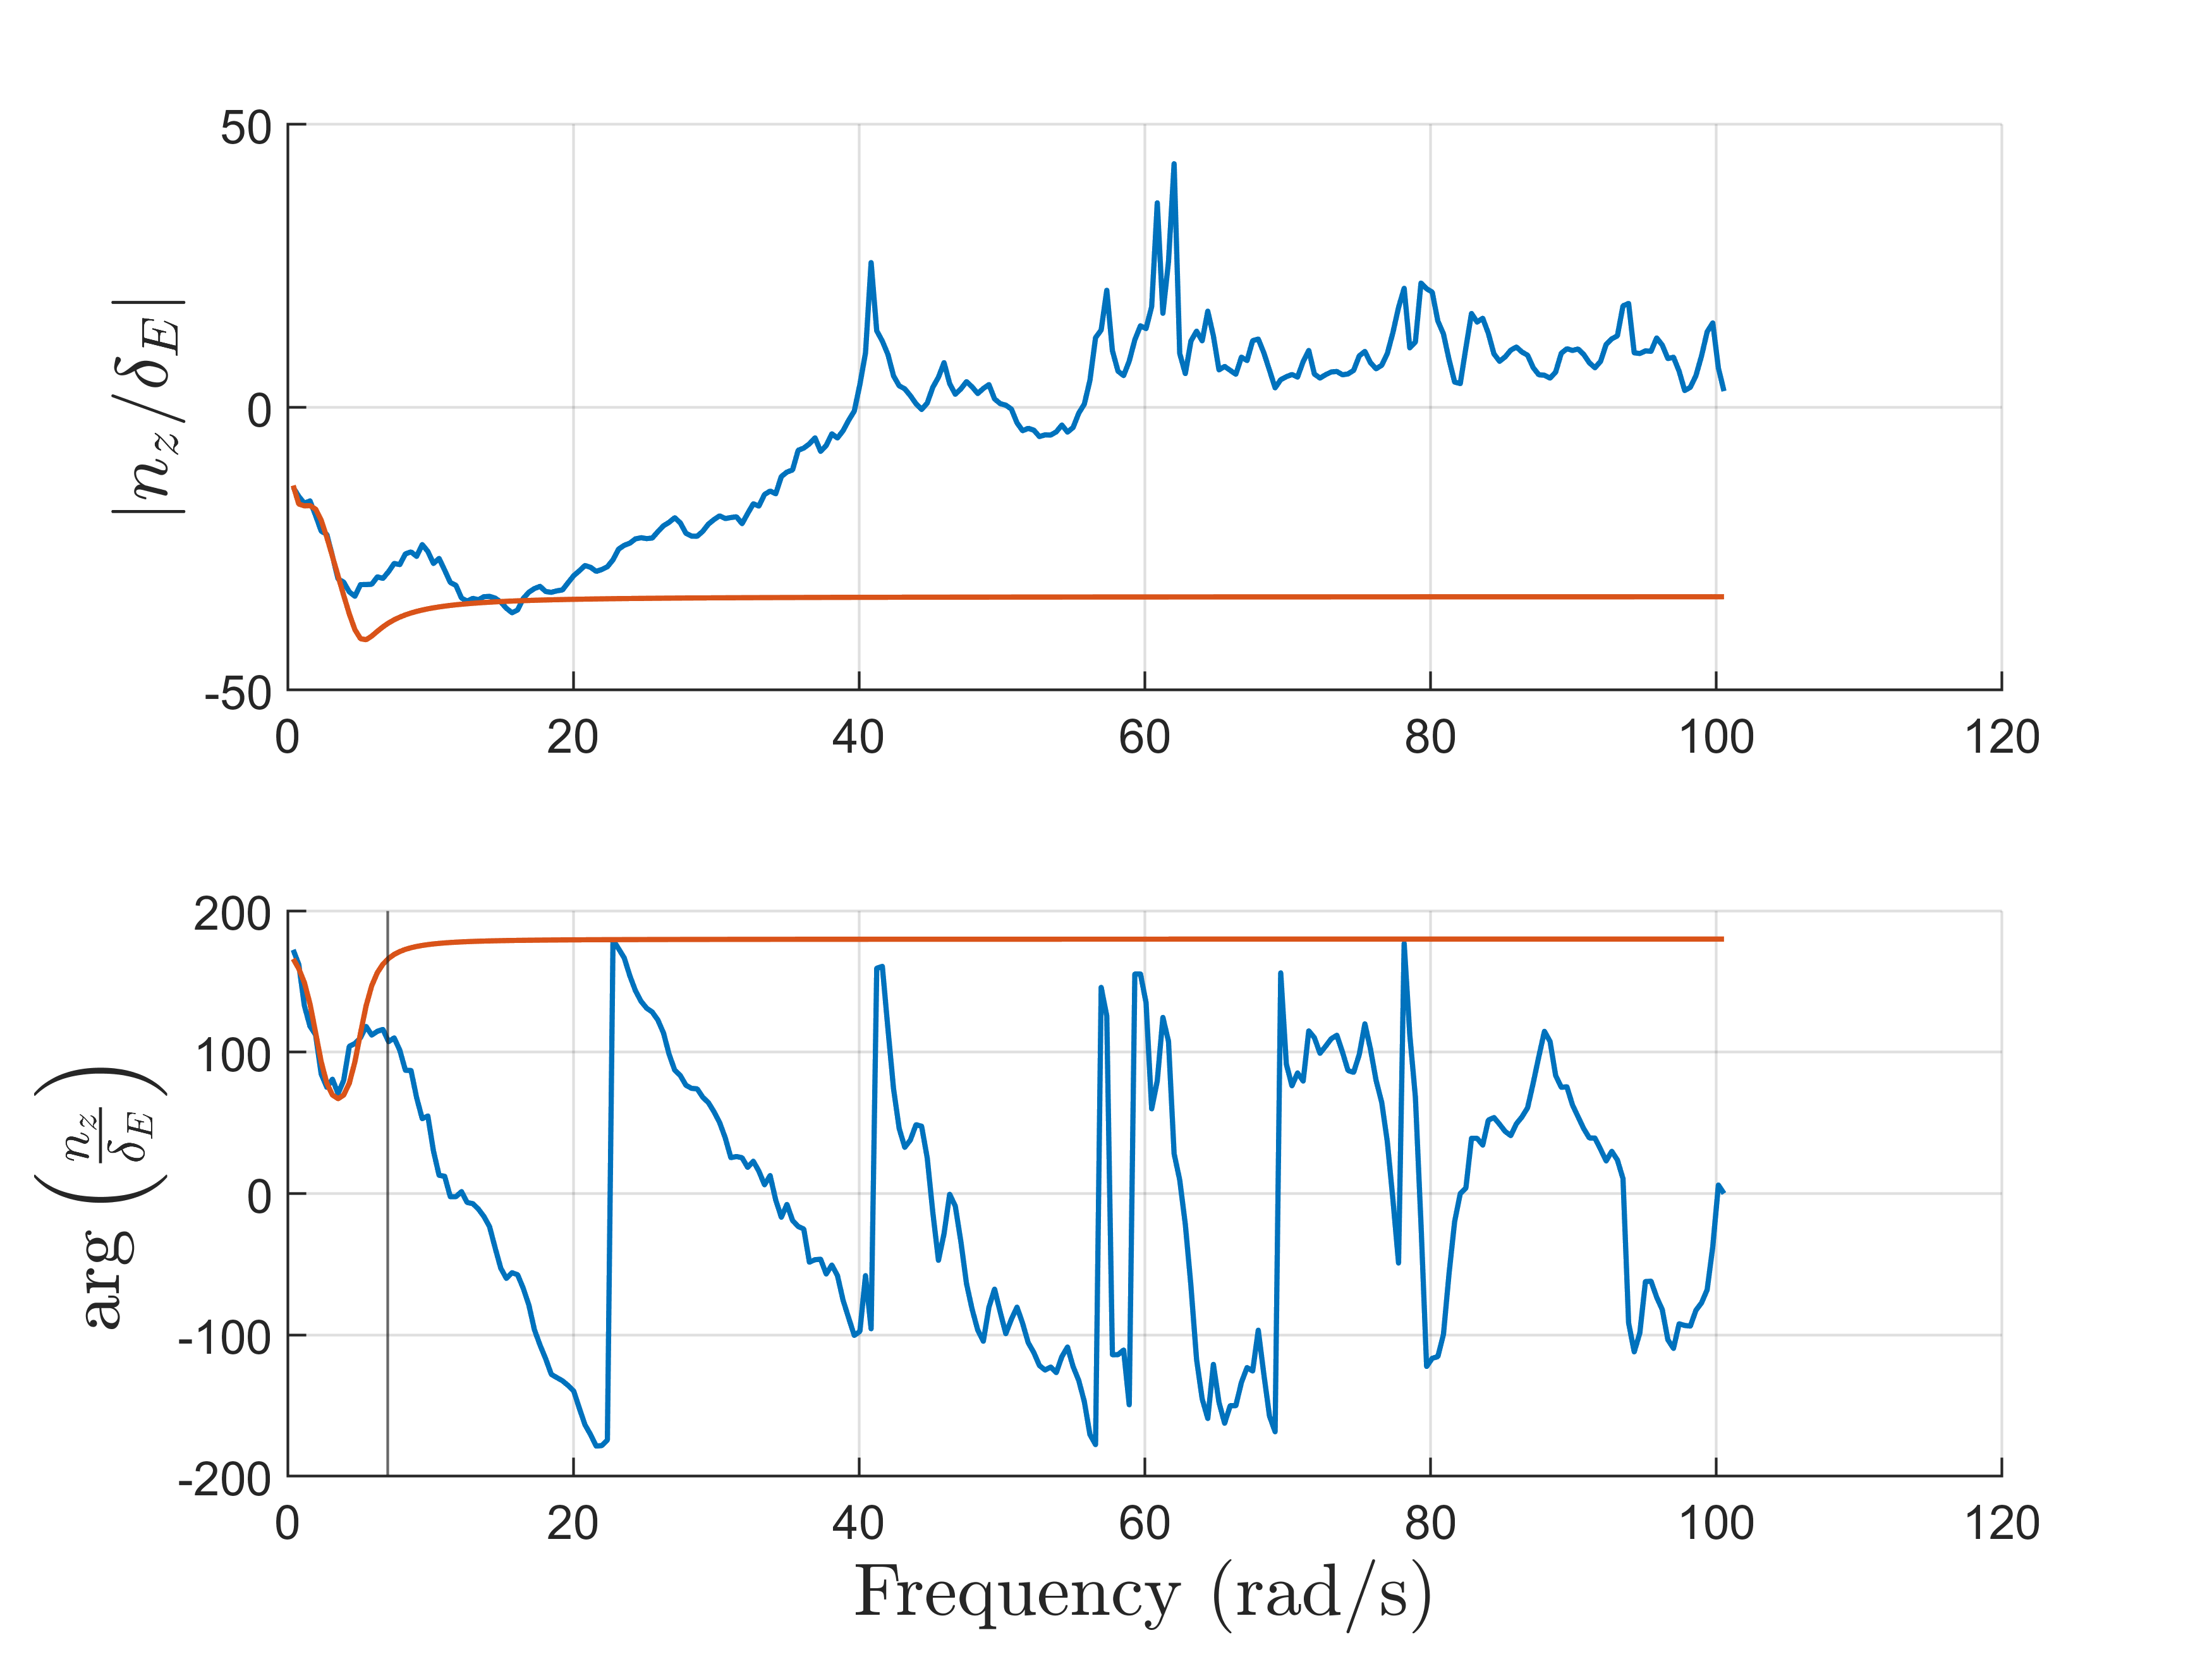
\includegraphics[width=0.6\textwidth]{elevator_to_normal.png}
      \caption{}
      \label{fig:elevator_to_normal}
  \end{figure}
  
  \begin{figure}[H]
      \centering
      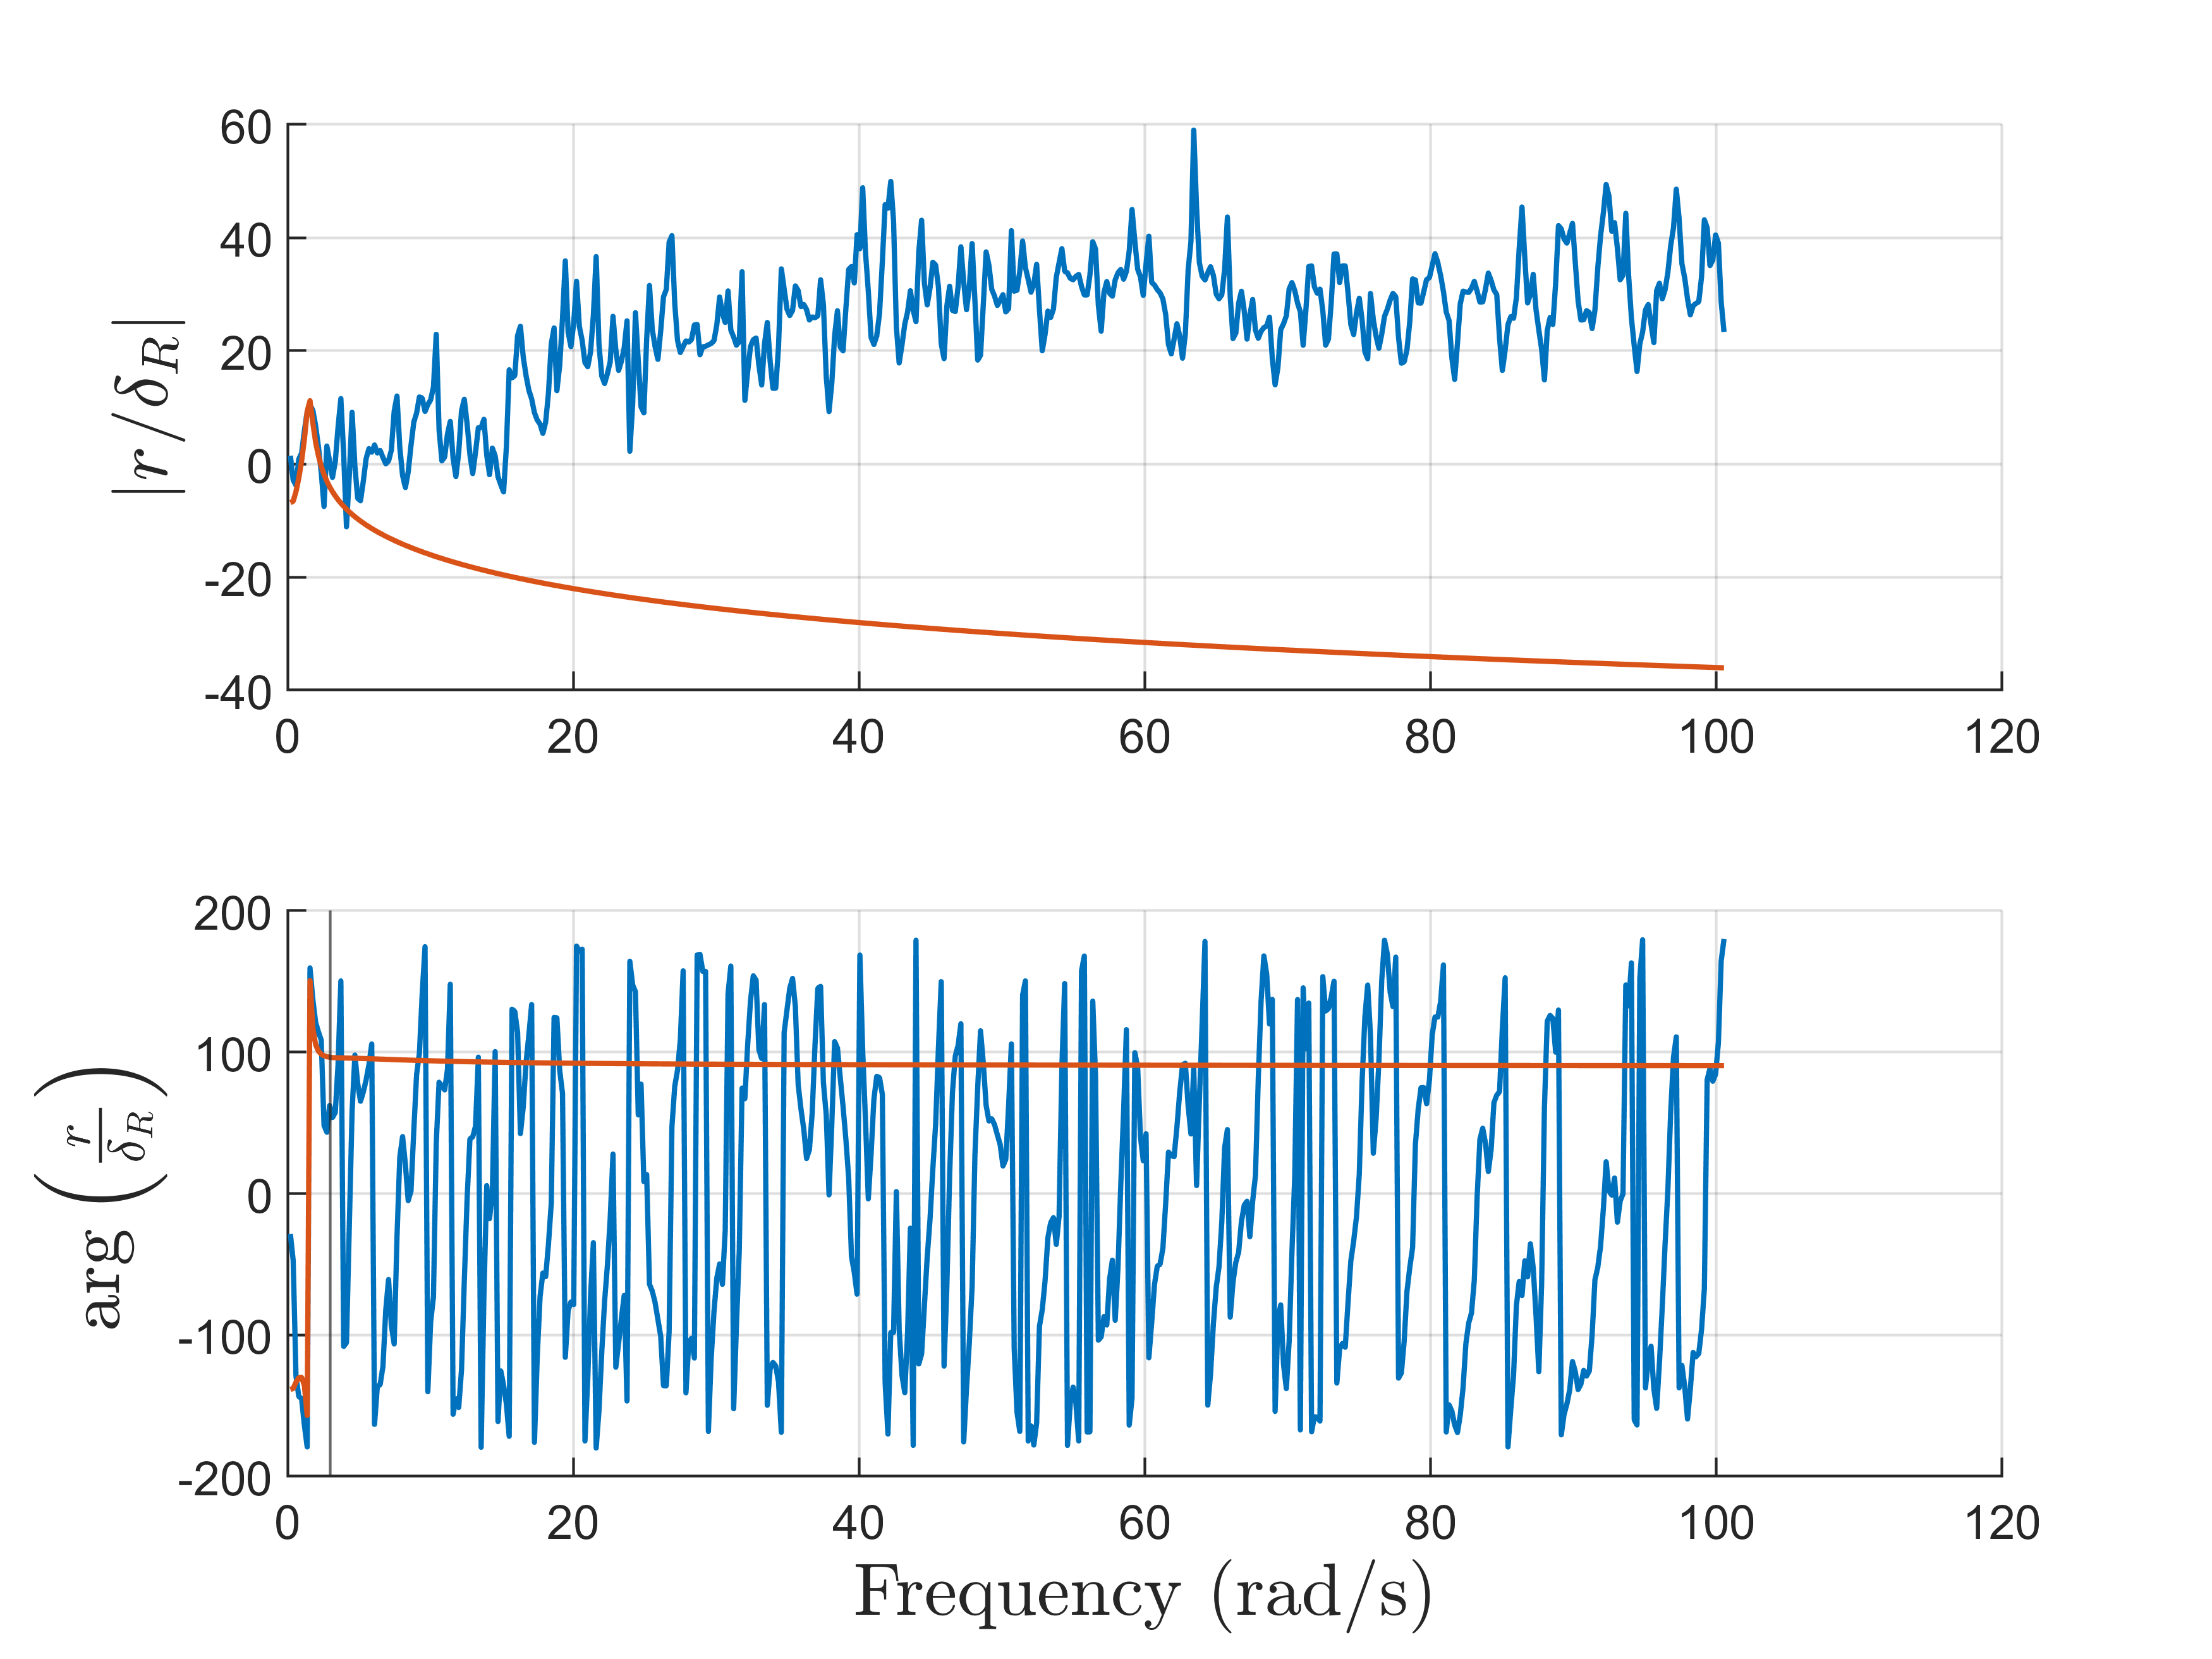
\includegraphics[width=0.6\textwidth]{rudder_to_yawrate.png}
      \caption{}
      \label{fig:rudder_to_yawrate}
  \end{figure}
  
  \begin{figure}[H]
      \centering
      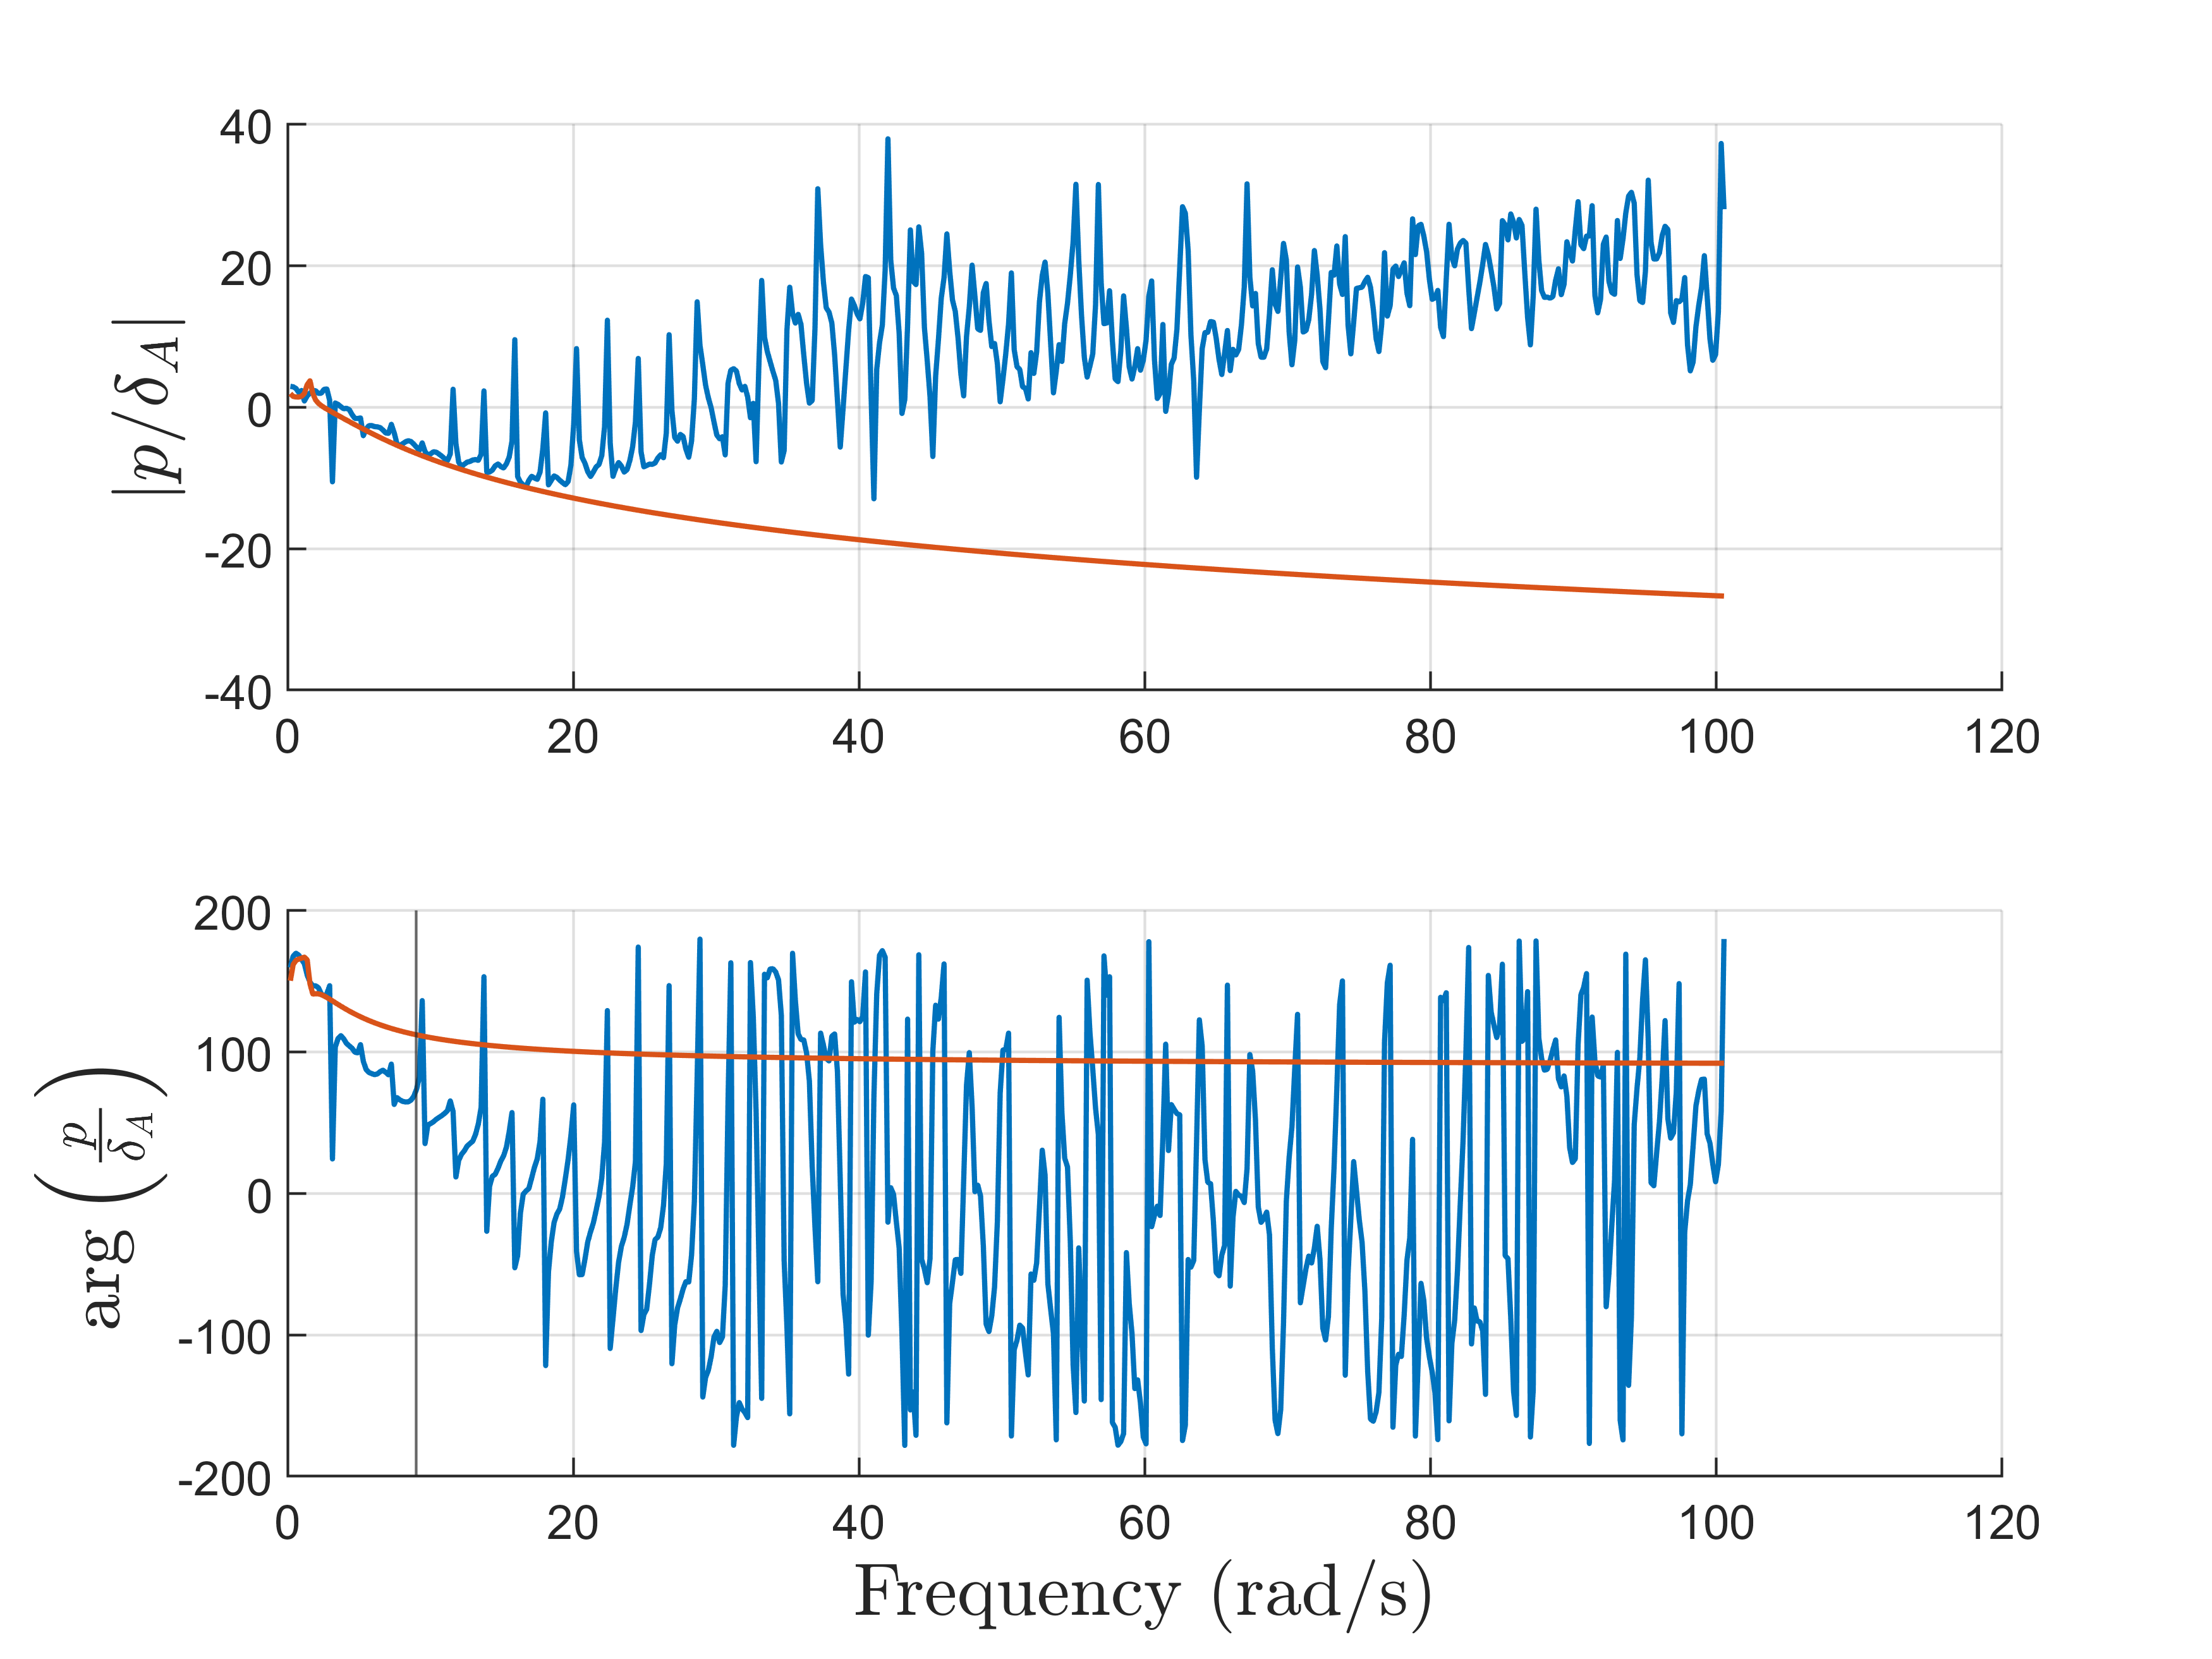
\includegraphics[width=0.6\textwidth]{aileron_to_rollrate.png}
      \caption{}
      \label{fig:aileron_to_rollrate}
  \end{figure}

\section{Transfer functions}

\begin{equation}
    \frac{\theta}{\delta_E} =
    -\frac{2.68513\,s^3+2.47159\,s^2+0.0889806\,s-0.212283}{s^4+1.63559\,s^3+3.41232\,s^2+0.079229\,s+0.0509983}
\end{equation}

\begin{equation}
    \frac{n_z}{\delta_E} =
    -\frac{0.0142876\,s^4+0.0729258\,s^3+0.405827\,s^2+0.0210445\,s-0.0283269}{s^4+1.63559\,s^3+3.41232\,s^2+0.079229\,s+0.0509983}
\end{equation}

\begin{equation}
    \frac{r}{\delta_R} =
    -\frac{1.15503\,s^3+6.7399\,s^2+1.55499\,s-0.316142}{s^4+4.44024\,s^3+4.02903\,s^2+9.1509\,s-0.217088}
\end{equation}

\begin{equation}
    \frac{\phi}{\delta_A} =
    -\frac{3.95865\,s^3+3.58235\,s^2+9.71187\,s+0.908058}{s^4+4.44024\,s^3+4.02903\,s^2+9.1509\,s-0.217088}
\end{equation}

\section{Conclusion}

\section{Appendix}

\begin{thebibliography}{9}

  \bibitem{handout}
  S. Place, A. Cooke
  \emph{Flight Experimental Methods: Course Handbook}
  Cranfield University,

  \bibitem{e2}
    5739G
    \emph{4A4 Exercise 2: Modal Analysis of SAAB 340B Flight Data}

\end{thebibliography}

\end{document}

